\section{Native Android Application
Structure}\label{native-android-application-structure}

A Native Android Application is composed of three main components:

\begin{itemize}
\tightlist
\item
  The resources like images and audio files required by the application
\item
  The code of the application
\item
  A manifest called the Android Manifest which describes the permissions
  required by the application, the entry-point of the application and
  the various activities which the application offer
\end{itemize}

An activity is a single page in the application which can show some
graphics elements called views.

An application can contain one or more activities and applications can
show different pages in the same activity by using a view called
Fragment which allows to easily define multiple layouts without using
multiple activities.

In order to access sensitive data and perform critical actions an
application must declare a permission in its Android Manifest and for
the most critical ones, obtain explicit permission from the user.

Applications are distributed using the apk file format which is a signed
zip.

\section{Common Android Malware
structure}\label{common-android-malware-structure}

Since in normal Android devices the user does not have access to the
root user and a privilege escalation requires the usage of a 0-day,
common Android malwares have to declare and obtain explicit permissions
from the user in order to have access to high value informations.

Between the available permissions, the most critical one is the
accessibility service, which allows an application to read the screen
content and perform actions on behalf of the user.

Google Play Store, the main application distribution system in the
Android ecosystem, performs strict checks over the applications' usage
of the declared permissions and this prevents malwares from declaring
the required permissions in their manifest.

To bypass the security checks of the Google Play Store malwares
typically open the system browser on a controlled link, this action
doesn't require any permission. On the controlled link a download of
another application immediately starts

\section{Security application scanner
architecture}\label{security-application-scanner-architecture}

A security application scanner typically is divided into three
components:

\begin{itemize}
\item
  the environment: which is a simulated environment as close as possible
  to the real environment in which the application under test is
  executed by the scanner to analyze the behaviour
\item
  the crawler: which interact and stimulated the application in order to
  explore as many different states as possible
\item
  the scanner: which analyzes the behaviour of the application during
  the crawler execution and interacts with it after the crawling to
  detect the vulnerabilities
\end{itemize}

\section{Current crawlers}\label{current-crawlers}

Crawlers while exploring the application build a model, which is a graph
containing as nodes the different states of the application and as edges
the actions performed to reach that state from a previous one. For
deciding the next edge to explore crawlers typically employ one or a
combination of these strategies:

\begin{itemize}
\tightlist
\item
  depth first search
\item
  breadth first search
\item
  random selection
\item
  weighted selections, where the weights are defined with a formula or
  by using reinforced learning models
\end{itemize}

\section{Crawling problem}\label{crawling-problem}

Mobile applications often have their main functionalities displayied in
deep states, this is due to the presence login screens and sequence of
steps which must be undertaken by the user.

The previous strategies are often not able to reach these deep states
due to their missing knowledge of common patterns in mobile
applications.

This limits the ability of dynamic security scanning tools to only
superficial states.

To solve this problem it is possible to employ large language models
since they pack together knowledge from common applications.

\section{YuraScanner}\label{yurascanner}

YuraScanner \autocite{yurascanner}, is an automated web dynamic
vulnerability scanner that employs large language models.

The architecture of the tool is the following:

\begin{figure}
\centering
\pandocbounded{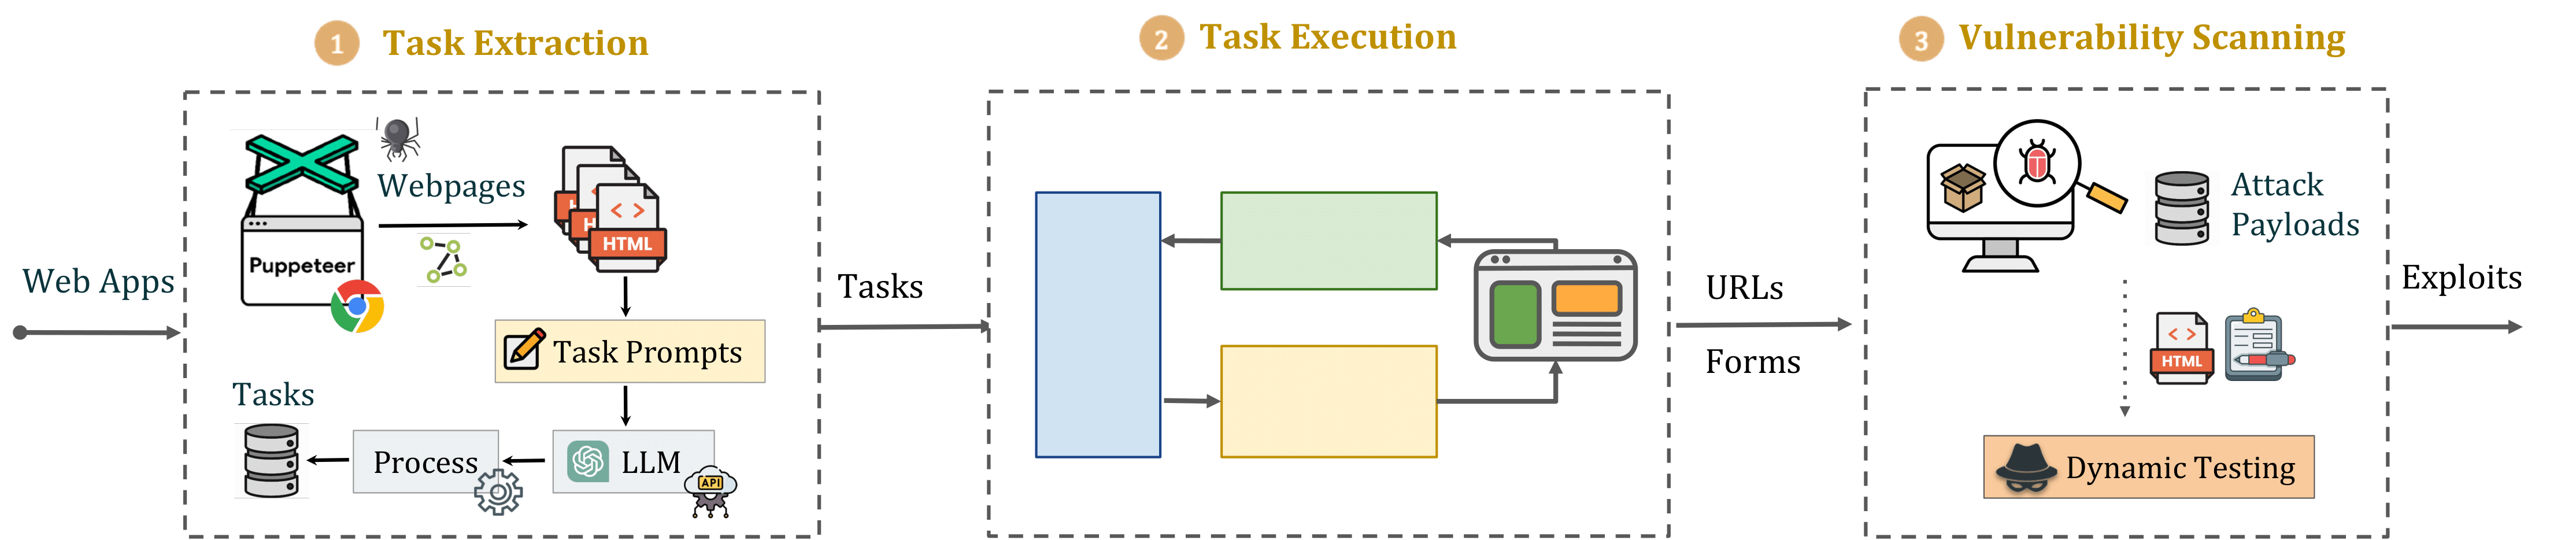
\includegraphics[keepaspectratio]{figs/yura.png}}
\caption{Overview of YuraScanner's architecture}
\end{figure}

Their architecture is divided into 3 major components: - Task extractor
- Task executor - Vulnerability scanning

\subsection{Task extractor}\label{task-extractor}

The task extractor component gets the HTML of the root page and the
pages immediately connected to the root page. The HTML is stripped from
non-textual and invisible components, and it is passed to a large
language model to generate a list of possible tasks to perform in the
application. The prompt used for the model is the following:

\begin{figure}
\centering
\pandocbounded{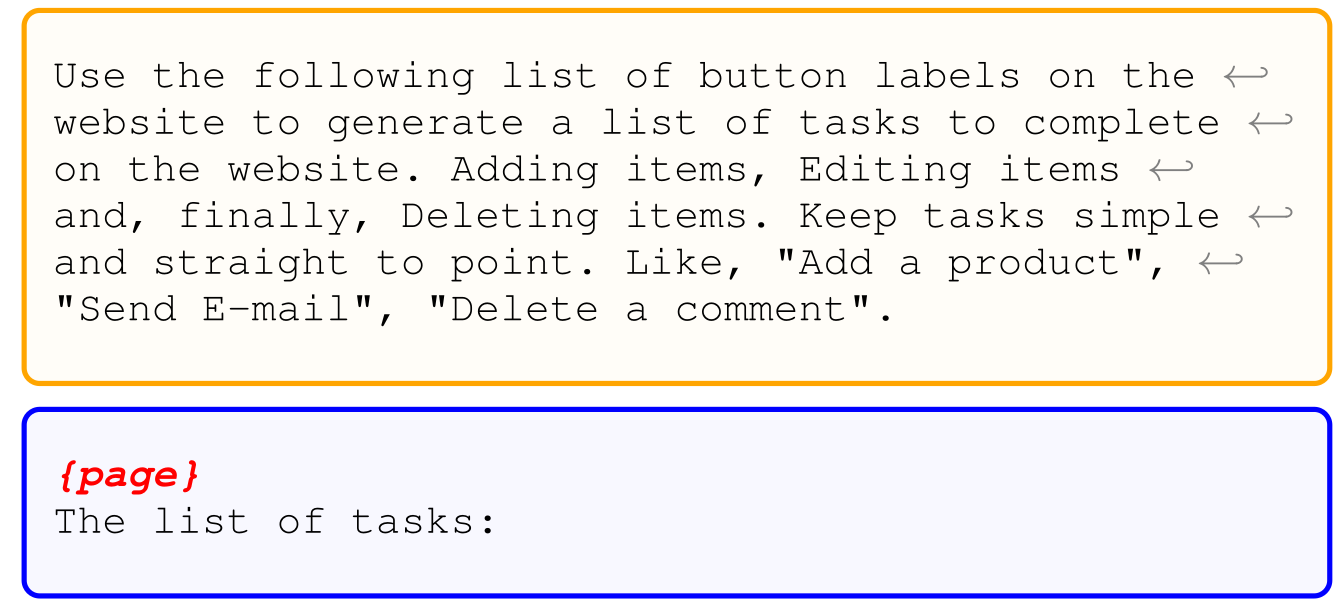
\includegraphics[keepaspectratio]{figs/extraction_prompt.png}}
\caption{Prompt for the tasks generation}
\end{figure}

\subsection{Task executor}\label{task-executor}

The task executor component takes a task as an input as is further
divided into the following components:

\begin{figure}
\centering
\pandocbounded{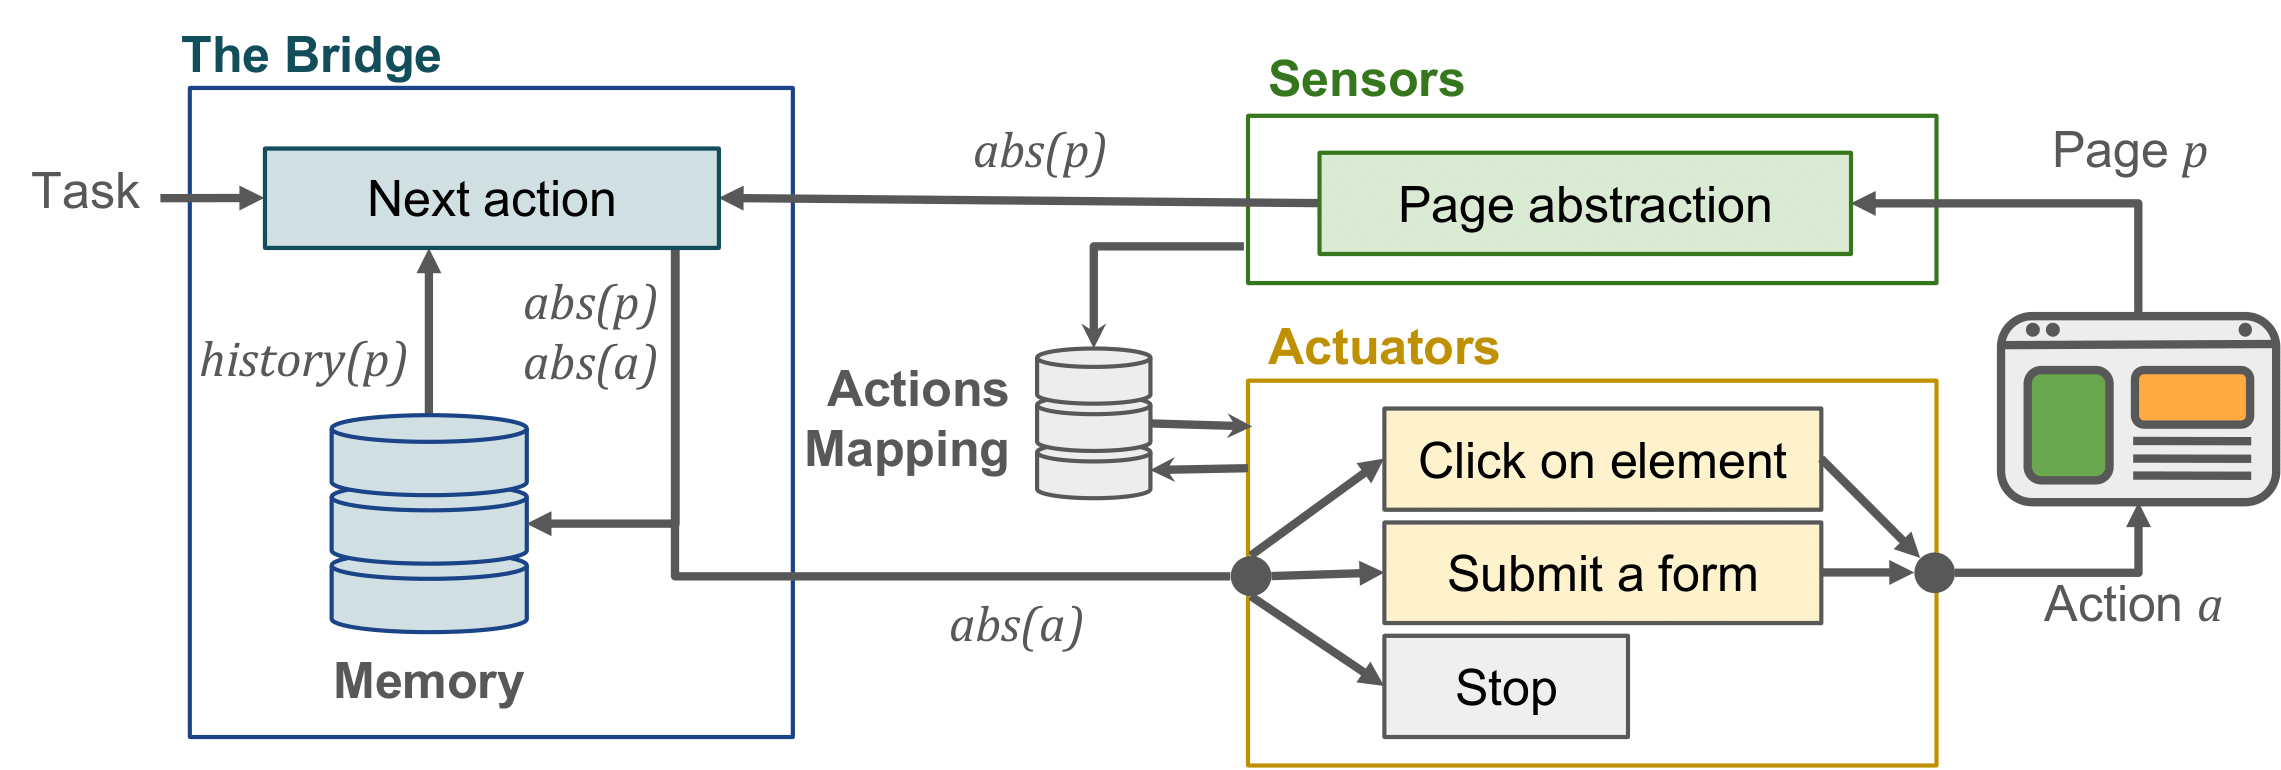
\includegraphics[keepaspectratio]{figs/execution.png}}
\caption{Task executor components}
\end{figure}

\subsubsection{Bridge}\label{bridge}

The bridge component uses the input task, an abstract representation of
the current page generated by the sensor component and a record of
previous actions to decide the next action to take. The prompt is
structured as following:

\begin{figure}
\centering
\pandocbounded{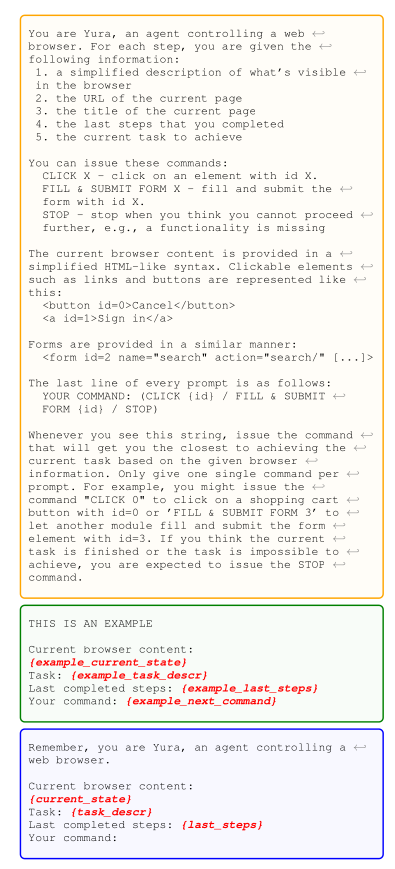
\includegraphics[keepaspectratio]{figs/execution_prompt.png}}
\caption{Prompt used for deciding the next action}
\end{figure}

The memory is a summary of the previous actions generated by the llm.
During each prompt in addition to the output, a summary of the previous
step plus the next one is asked to the model and replaces the previous
text in the memory.

\subsubsection{Actuators}\label{actuators}

The selected next action is passed to the actuator which applies it to
the environment, in this case by using puppeteer for automating browser
actions. When the stop action is issued the task executor stops and
proceeds to a new task.

\subsubsection{Sensors}\label{sensors}

The sensor component extracts the HTML of the current visualized page
using puppeteer and creates and an abstraction for it by stripping non
interactable and invisible elements.

\subsection{Vulnerability scanner}\label{vulnerability-scanner}

The vulnerabily scanner component uses a set of collected urls and forms
to perform on them further analysis using attack modules for finding
common vulnerabilities.

\subsection{Notes}\label{notes}

YuraScanner solves the crawling problem by generating a list of possible
tasks from the home pages and then execute them using a browser
automation agent powered by the llm. An llm is capable of completing
this task since llms have knowledge of common application workflows due
to their large input dataset.

\section{AppAgent}\label{appagent}

AppAgent \autocite{yang2023appagent} is an automated agent for Android
devices powered by OpenAi.

\begin{figure}
\centering
\pandocbounded{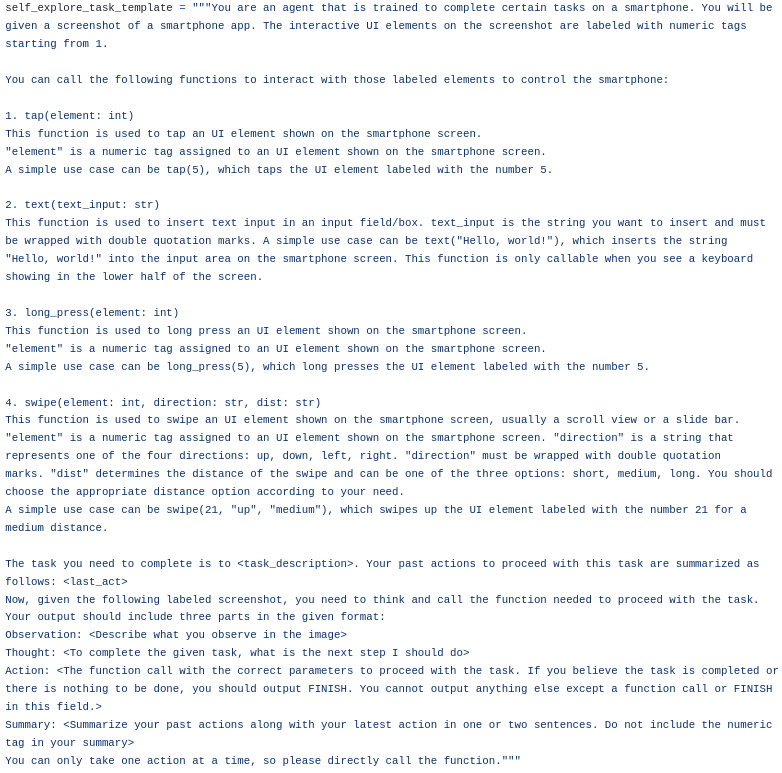
\includegraphics[keepaspectratio]{figs/appagent_prompt.png}}
\caption{Prompt used by AppAgent}
\end{figure}

AppAgent compared to YuraScanner uses multimodal models instead of text
only models. A screenshot of the device is taken and numbered labels are
added to each interactive element in the screenshot. For generating the
labels an XML dump of the layout is obtained by using the adb dump
utility. The llm then chooses the action and the element to execute it
on based on the labels in the image. The process terminates when a
certain number of steps is reached or when the model calls the finish
action. AppAgent isn't an autonomous cralwer since it requires an input
task to perform.
